\documentclass{article}%
\usepackage[T1]{fontenc}%
\usepackage[utf8]{inputenc}%
\usepackage{lmodern}%
\usepackage{textcomp}%
\usepackage{lastpage}%
\usepackage[head=40pt,margin=0.5in,bottom=0.6in]{geometry}%
\usepackage{graphicx}%
%
\title{\textbf{Denunciaron que propietario de farmacia en Amazonas tiene 30 días detenido}}%
\author{El Nacional Web}%
\date{23/09/2018}%
%
\begin{document}%
\normalsize%
\maketitle%
\textbf{URL: }%
http://www.el{-}nacional.com/noticias/sociedad/denunciaron{-}que{-}propietario{-}farmacia{-}amazonas{-}tiene{-}dias{-}detenido\_252957\newline%
%
\textbf{Periodico: }%
EN, %
ID: %
252957, %
Seccion: %
Sociedad\newline%
%
\textbf{Palabras Claves: }%
Amazonas, Sociedad\newline%
%
\textbf{Derecho: }%
1.2%
, Otros Derechos: %
2.1%
, Sub Derechos: %
1.2.1.3, 2.1.1%
\newline%
%
\textbf{EP: }%
NO\newline%
\newline%
%
\textbf{\textit{El dirigente político Liborio Guarulla aseguró que el detenido, junto a su esposa, colaboraron activamente en el auxilio de ciudadanos durante la emergencia por inundaciones en el estado}}%
\newline%
\newline%
%
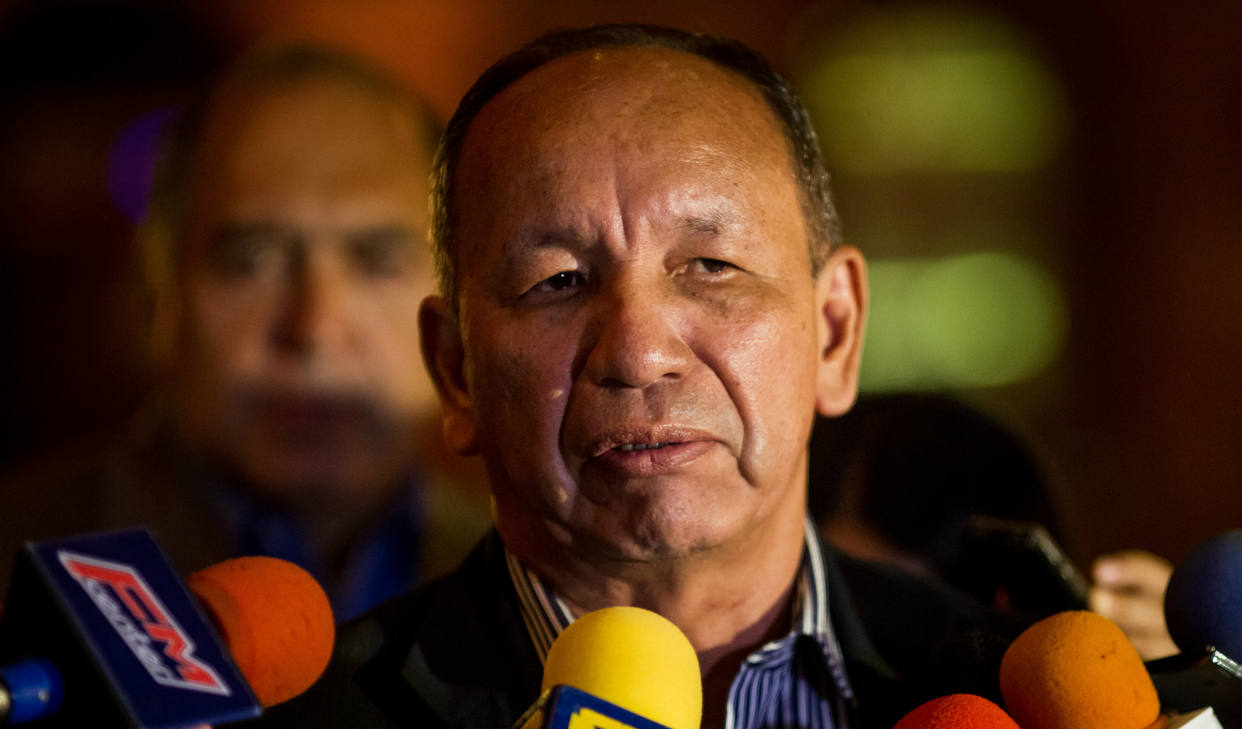
\includegraphics[width=300px]{145.jpg}%
\newline%
%
Liborio Guarulla, ex gobernador del estado Amazonas, denunció este domingo que el copropietario de la farmacia Autana lleva 30 días preso. Los funcionarios de seguridad que apresaron al comerciante alegaron "conmoción social".%
\newline%
%
"Carlos Acevedo, copropietario de la farmacia Autana en Puerto Ayacucho, lleva 30 días preso por 'orden superior'~de Maduro y el Servicio Bolivariano de Inteligencia (Sebin),~por 'conmoción social'", indicó el ex gobernador en Twitter.%
\newline%
%
El dirigente político aseguró que el detenido, junto a su esposa, colaboraron activamente en el auxilio de ciudadanos durante la emergencia por inundaciones en el estado.%
\newline%
%
"La verdad es que junto a su esposa~fueron los que más salvaron vidas durante la emergencia por inundaciones en Amazonas", aseveró Guarulla.%
\newline%
%
\end{document}